\begin{figure}[htb]
    \begin{mdframed}
    \begin{tikzpicture}

        \begin{scope}
            
% Population
\node [box] (population) {};
\node [anchor=north] at (population.north) {Population};

\node (line1) [anchor=south west] at (population.south west) {$\coloredrule{10mm}{1mm}{green!50}$};
\node (line2) [anchor=south west] at (line1.south east) {$\coloredrule{10mm}{1mm}{red!25}$};
\node (line3) [anchor=south west] at (line2.south east) {$\coloredrule{10mm}{1mm}{blue!50}$};
\node (line4) [anchor=south west] at (line1.north west) {$\coloredrule{10mm}{1mm}{red!50}$};
\node (line5) [anchor=south west] at (line2.north west) {$\coloredrule{10mm}{1mm}{lime!50}$};
\node (line6) [anchor=south west] at (line3.north west) {$\coloredrule{10mm}{1mm}{blue!75}$};
\node (line7) [anchor=south west] at (line4.north west) {$\coloredrule{10mm}{1mm}{blue!25}$};
\node (line8) [anchor=south west] at (line5.north west) {$\coloredrule{10mm}{1mm}{red!75}$};
\node (line9) [anchor=south west] at (line6.north west) {$\coloredrule{10mm}{1mm}{teal!50}$};

        \end{scope}

        \begin{scope}[xshift=4.6cm]
            
\begin{tikzpicture}
    \tikzstyle{box} = [rectangle, rounded corners, minimum width=4cm, minimum height=1.8cm,text centered, draw=black, fill=gray!10]

    % Phenotypes
    \node [box] (phenotypes) {};
    \node [anchor=north] at (phenotypes.north) {phenotypes};
    \node (phenotype1) [anchor=south west] at (phenotypes.south west) {\resizebox{0.05\textwidth}{!}{\def\layersep{2.5cm}

\begin{tikzpicture}[shorten >=1pt,->,draw=black!50, node distance=\layersep]
    \tikzstyle{every pin edge}=[<-,shorten <=1pt]
    \tikzstyle{neuron}=[circle,fill=black!25,minimum size=17pt,inner sep=0pt]
    \tikzstyle{input neuron}=[neuron, fill=green!50];
    \tikzstyle{output neuron}=[neuron, fill=red!50];

    % Draw the input nodes.
    \foreach \name / \y in {1,...,2}
        \node[input neuron] (I-\name) at (0,-\y) {};

    % Draw the output node.
    \node[output neuron, right of=H-2] (O-1) {};

    % Connect inputs with output node.
    \draw (I-1) -- (O-1);
    \draw (I-2) -- (O-1);
\end{tikzpicture}}};
    %\node (phenotype2) [anchor=south west] at (phenotype1.south west) {\resizebox{0.05\textwidth}{!}{\def\layersep{2.5cm}

\begin{tikzpicture}[shorten >=1pt,->,draw=black!50, node distance=\layersep]
    \tikzstyle{every pin edge}=[<-,shorten <=1pt]
    \tikzstyle{neuron}=[circle,fill=black!25,minimum size=17pt,inner sep=0pt]
    \tikzstyle{input neuron}=[neuron, fill=green!50];
    \tikzstyle{output neuron}=[neuron, fill=red!50];

    % Draw the input nodes.
    \foreach \name / \y in {1,...,2}
        \node[input neuron] (I-\name) at (0,-\y) {};

    % Draw the output node.
    \node[output neuron, right of=H-2] (O-1) {};

    % Connect inputs with output node.
    \draw (I-1) -- (O-1);
    \draw (I-2) -- (O-1);
\end{tikzpicture}}};
    %\node (phenotype3) [anchor=south west] at (phenotype2.south west) {\resizebox{0.05\textwidth}{!}{\def\layersep{2.5cm}

\begin{tikzpicture}[shorten >=1pt,->,draw=black!50, node distance=\layersep]
    \tikzstyle{every pin edge}=[<-,shorten <=1pt]
    \tikzstyle{neuron}=[circle,fill=black!25,minimum size=17pt,inner sep=0pt]
    \tikzstyle{input neuron}=[neuron, fill=green!50];
    \tikzstyle{output neuron}=[neuron, fill=red!50];

    % Draw the input nodes.
    \foreach \name / \y in {1,...,2}
        \node[input neuron] (I-\name) at (0,-\y) {};

    % Draw the output node.
    \node[output neuron, right of=H-2] (O-1) {};

    % Connect inputs with output node.
    \draw (I-1) -- (O-1);
    \draw (I-2) -- (O-1);
\end{tikzpicture}}};
\end{tikzpicture}
        \end{scope}

        \begin{scope}[xshift=9.8cm, yshift=-0.04cm, every node/.append style={transform shape}]
            \tikzstyle{box} = [rectangle, rounded corners, minimum width=4.7cm, minimum height=2.2cm,text centered, draw=black, fill=white!10]
            \node [box] (evaluation) {};
            \node [anchor=north] at (evaluation.north) {Evaluation};
        \end{scope}

        \begin{scope}[xshift=8.8cm, yshift=-0.04cm, scale=0.6, every node/.append style={transform shape}]
            
\node [box] (evaluation) {};
\node [anchor=north] at (evaluation.north) {Evaluation};


        \end{scope}

        \begin{scope}[xshift=10cm, yshift=-2.6cm]
            
\node [box] (speciate) {};
\node [anchor=north] at (speciate.north) {Speciation};

\node (line1) [anchor=south west] at (speciate.south west) {$\coloredrule{10mm}{1mm}{OliveGreen}$};
\node (line2) [anchor=south west] at (line1.south east) {$\coloredrule{10mm}{1mm}{RubineRed}$};
\node (line3) [anchor=south west] at (line2.south east) {$\coloredrule{10mm}{1mm}{blue}$};
\node (line4) [anchor=south west] at (line1.north west) {$\coloredrule{10mm}{1mm}{green}$};
\node (line5) [anchor=south west] at (line2.north west) {$\coloredrule{10mm}{1mm}{red}$};
\node (line6) [anchor=south west] at (line3.north west) {$\coloredrule{10mm}{1mm}{Periwinkle}$};
\node (line7) [anchor=south west] at (line4.north west) {$\coloredrule{10mm}{1mm}{SeaGreen}$};
\node (line8) [anchor=south west] at (line5.north west) {$\coloredrule{10mm}{1mm}{Salmon}$};
\node (line9) [anchor=south west] at (line6.north west) {$\coloredrule{10mm}{1mm}{Cyan}$};


        \end{scope}

        \begin{scope}[xshift=7.5cm, yshift=-5cm]
            
\node [box] (selection) {};
\node [anchor=north] at (selection.north) {Selection};

\node (line1) [anchor=south west] at (selection.south west) {$\coloredrule{10mm}{1mm}{OliveGreen}$};
\node (line2) [anchor=south west] at (line1.south east) {$\coloredrule{10mm}{1mm}{Red}$};
\node (line3) [anchor=south west] at (line2.south east) {$\coloredrule{10mm}{1mm}{blue}$};
\node (line4) [anchor=south west] at (line1.north west) {$\coloredrule{10mm}{1mm}{green}$};
\node (line5) [anchor=south west] at (line2.north west) {$\coloredrule{10mm}{1mm}{Salmon}$};
\node (line6) [anchor=south west] at (line3.north west) {$\coloredrule{10mm}{1mm}{Periwinkle}$};

        \end{scope}

        \begin{scope}[xshift=2.5cm, yshift=-5cm]
            

\node [box] (reproduction) {};
\node [anchor=north] at (reproduction.north) {Reproduction};

\node (line1) [anchor=south west] at (reproduction.south west) {$\coloredrule{10mm}{1mm}{OliveGreen, green}$};
\node (line2) [anchor=south west] at (line1.south east) {$\coloredrule{10mm}{1mm}{red, Salmon}$};
\node (line3) [anchor=south west] at (line2.south east) {$\coloredrule{10mm}{1mm}{blue, Periwinkle}$};
\node (line4) [anchor=south west] at (line1.north west) {$\coloredrule{10mm}{1mm}{green, OliveGreen}$};
\node (line5) [anchor=south west] at (line2.north west) {$\coloredrule{10mm}{1mm}{Salmon, red}$};
\node (line6) [anchor=south west] at (line3.north west) {$\coloredrule{10mm}{1mm}{Periwinkle, blue}$};
\node (line7) [anchor=south west] at (line4.north west) {$\coloredrule{10mm}{1mm}{green}$};
\node (line8) [anchor=south west] at (line5.north west) {$\coloredrule{10mm}{1mm}{red}$};
\node (line9) [anchor=south west] at (line6.north west) {$\coloredrule{10mm}{1mm}{blue}$};
        \end{scope}

        \begin{scope}[xshift=0cm, yshift=-2.6cm]
            
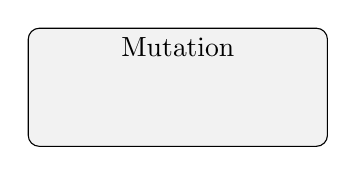
\begin{tikzpicture}
    \tikzstyle{box} = [rectangle, rounded corners, minimum width=3.8cm, minimum height=1.5cm,text centered, draw=black, fill=gray!10]

    \node [box] (mutation) {};
    \node [anchor=north] at (mutation.north) {Mutation};

    % TODO: slightly shift the color of the offspring.

  \end{tikzpicture}
        \end{scope}

        \draw[-latex, thick, shorten >=0.1cm, shorten <=0.1cm] (population) -- (phenotypes);
        \draw[-latex, thick, shorten >=0.1cm, shorten <=0.2cm] (phenotypes.east) -- (evaluation);
        \draw[-latex, thick,shorten >=0.1cm, shorten <=0.1cm] (evaluation) -- (speciate);
        \draw[-latex, thick, shorten >=0.2cm, shorten <=0.2cm] (speciate) -- (selection);
        \draw[-latex, thick, shorten >=0.2cm, shorten <=0.2cm] (selection) -- (reproduction);
        \draw[-latex, thick, shorten >=0.2cm, shorten <=0.2cm] (reproduction) -- (mutation);
        \draw[-latex, thick,shorten >=0.1cm, shorten <=0.1cm] (mutation) -- (population);

    \end{tikzpicture}
    \end{mdframed}
    \caption{Overview of the NEAT algorithm, proceeding clockwise from the population-box in
    the upper left corner.}
\end{figure}